\documentclass[conference]{IEEEtran}

\usepackage{graphicx}
\usepackage{amsmath}
\usepackage{amssymb}
\usepackage{booktabs}
\usepackage{xcolor}
\usepackage{hyperref}
\usepackage{siunitx}
\usepackage{multirow}
\usepackage{subcaption}
\usepackage[font=small]{caption}
\usepackage{pifont}

\hypersetup{
  colorlinks=true,
  linkcolor=black,
  citecolor=[rgb]{0.0,0.35,0.65},
  urlcolor=[rgb]{0.0,0.35,0.65}
}

\title{Sensorless Bilateral Force Feedback for\\Low-Cost Scaled Teleoperation}

\author{\IEEEauthorblockN{Leonardo Camacho Pel\'{a}ez}
\IEEEauthorblockA{University of Edinburgh\\
\texttt{leocamacho707@gmail.com}}}

\makeatletter
\ifCLASSOPTIONconference
\def\@maketitle{\newpage
\bgroup\par\vskip\IEEEtitletopspace\vskip\IEEEtitletopspaceextra\centering%
   \vskip0.2em{\Huge\ifCLASSOPTIONtransmag\bfseries\LARGE\fi\@IEEEcompsoconly{\sffamily}\@IEEEcompsocconfonly{\normalfont\normalsize\vskip 2\@IEEEnormalsizeunitybaselineskip
   \bfseries\Large}\@IEEEcompsocnotconfonly{\vskip 0.75\@IEEEnormalsizeunitybaselineskip}\@title\par}\relax
   \@IEEEcompsocnotconfonly{\vskip 0.5\@IEEEnormalsizeunitybaselineskip}\vskip1.0em\par%
   {\@IEEEspecialpapernotice\mbox{}\vskip\@IEEEauthorblockconfadjspace%
    \mbox{}\hfill\begin{@IEEEauthorhalign}\@author\end{@IEEEauthorhalign}\hfill\mbox{}\par}\relax
   \vskip 1.2em
   \begin{minipage}{\textwidth}
      \centering
      \includegraphics[width=\textwidth]{figures/hero.png}
      \par\vspace{0.35em}
      {\footnotesize Fig.~1: \textbf{System overview.} (A)~The operator controls a PincherX-100 leader arm while the 2$\times$-scaled follower contacts an obstacle. (B)~Motor effort readings from the follower arm during obstacle contact: shoulder effort (dark) exceeds the 300\,mA feedback threshold (dashed), triggering proportional resistance at the leader. (C)~RViz visualisation showing leader and follower arm states in real time.\par}
   \end{minipage}\par
\par\addvspace{0.5\baselineskip}\egroup}
\fi
\makeatother

\begin{document}

\maketitle
\setcounter{figure}{0}
\refstepcounter{figure}\label{fig:hero}

% ===== ABSTRACT =====
\begin{abstract}
We present a bilateral teleoperation system in which two small commodity leader arms control two 3D-printed follower arms at twice the scale.
The followers use torque-tiered actuators---high-torque motors only at joints that demand them---saving 55\% on motor costs.
The complete four-arm platform costs approximately \$3{,}000, an order of magnitude less than comparable systems.
Unlike recent low-cost platforms (ALOHA, GELLO, Koch arm), ours provides force feedback: the leader arm experiences resistance when the follower contacts an object.
This is achieved exclusively using motor current as a force proxy, with no dedicated sensors.
In a study with 22 participants, operators detected real obstacles through force feedback with 91\% mean sensitivity and rated learnability at the maximum score (median 7/7).
The primary limitation is that motor current cannot distinguish gravity from contact---an extended arm produces the same signal as a collision.
We tested three alternative feedback policies to resolve this; each failed for a different physical reason, confirming that a dynamics model is required.
All source code, CAD files, and hardware documentation are released as open source at \url{https://leocamacho.co/teleop}.
\end{abstract}

% ===== INTRODUCTION =====
\section{Introduction}

In 1949, Raymond Goertz built the first mechanical bilateral manipulator at Argonne National Laboratory, allowing a human operator to handle radioactive materials while feeling the forces encountered by the remote arm~\cite{goertz1949}. Five years later, Goertz replaced the mechanical linkage with electrical servo coupling~\cite{goertz1954}, establishing the fundamental architecture that bilateral teleoperators still follow today: a leader arm that the operator moves, a follower arm that tracks it, and a feedback channel that communicates environment forces back to the operator's hand.

For decades, this architecture required industrial-grade hardware. A recent wave of low-cost systems has begun to change this. ALOHA~\cite{zhao2023aloha} demonstrated fine bimanual manipulation for approximately \$20,000 using commodity arms. GELLO~\cite{wu_2024_gello} built kinematically-matched leaders for under \$300. The Koch arm~\cite{koch2024} pushed the cost of a single leader-follower pair below \$250. These systems have enabled imitation learning at previously impossible scale.

However, all of these systems are \emph{unilateral}: the operator moves the leader, the follower tracks, and that is all. There is no force feedback channel. The reason is straightforward: bilateral control traditionally requires force/torque sensors (\$4,000--10,000 each) or carefully calibrated dynamics models. Neither is practical on commodity servo hardware. Recent concurrent work has begun to explore this gap~\cite{echo2025, sujit_2025_improving, kobayashi2024, kanai2025}, but a complete, low-cost bilateral system with custom-scaled hardware and an honest characterisation of its limits has been lacking.

We present a system that closes this gap by using motor current as a force proxy. Our contributions are:

\begin{enumerate}
    \item \textbf{Sensorless bilateral force feedback} on commodity Dynamixel servos, using motor current readings as a proportional force proxy. We achieve 91.1\% obstacle detection sensitivity in a user study without any dedicated force sensors. We characterise the electromagnetic braking effect that makes naive implementations fail.

    \item \textbf{Custom 2$\times$-scaled follower arms} with 3D-printed links and a torque-tiered motor configuration (high-torque XM430 at shoulder/elbow, low-torque XL430 elsewhere), reducing per-follower motor cost by 55\% versus a uniform design.

    \item \textbf{A complete dual-pair bimanual system} at $\sim$\$3,000 total---an order of magnitude cheaper than ALOHA---with collision avoidance, graceful shutdown, smooth startup, and shared autonomy.

    \item \textbf{An empirical characterisation of the gravity-contact ambiguity}: we evaluate three alternative feedback policies for handling gravity-induced false positives, each failing for a distinct physical reason, and identify model-based gravity compensation as the established solution.
\end{enumerate}

All hardware designs, source code, and CAD files are publicly available.\footnote{\url{https://github.com/theCampel/sensorless-bilateral-teleop}}

% ===== RELATED WORK =====
\section{Related Work}

\subsection{Low-Cost Teleoperation}

The past two years have seen rapid progress in accessible teleoperation. ALOHA~\cite{zhao2023aloha} paired ViperX-300 followers with custom Dynamixel-based leaders for bimanual manipulation, enabling Action Chunking with Transformers (ACT) for imitation learning. GELLO~\cite{wu_2024_gello} built 3D-printed kinematically-matched leaders for Franka, UR5, and xArm followers at under \$300 per leader. The Koch arm~\cite{koch2024} demonstrated that a single pair could be built for under \$250. U-ARM~\cite{zou_2025_uarm} and LeRobot~\cite{lerobot2025} further pushed accessibility.

All of these systems are unilateral. The operator sends commands; the follower executes them; there is no return channel. Our work adds bilateral force feedback to this class of system using only the hardware already present.

\subsection{Bilateral Control}

Bilateral teleoperation has a long theoretical history. Lawrence~\cite{lawrence_1993_stability} established the fundamental stability-transparency trade-off: perfect force transparency requires infinite controller stiffness, which is inherently destabilising. The four-channel bilateral architecture~\cite{hokayem2006} and wave variable methods~\cite{anderson1989} address time-delay stability but assume force sensing at both ends. Impedance control~\cite{hogan1985} provides a framework for contact interaction but again typically requires force measurements.

On commodity servo hardware, dedicated force sensors are impractical. Recent concurrent work has begun exploring sensorless alternatives: GELLO+Force~\cite{sujit_2025_improving} augments GELLO with strain-gauge-based force sensing on a Franka Panda, Bi-ACT~\cite{kobayashi2024} demonstrates the importance of bilateral feedback for imitation learning quality using disturbance observers at 1\,kHz, Echo~\cite{echo2025} proposes open-source force feedback, and IGBT~\cite{kanai2025} achieves sensorless bilateral control by clamping leader commands by follower effort magnitude. Our work differs in using only the motor current readings already available on standard Dynamixel servos, requiring no additional sensing hardware, and in building custom-scaled followers rather than using commercial off-the-shelf arms.

\subsection{Motor Current as Force Proxy}

Using motor current (or torque) as a proxy for external forces is well-established in industrial robotics~\cite{morante2016}. The approach works because motor current is proportional to torque output, which includes both the desired motion torque and any external disturbance. Matsumoto et al.~\cite{fast_bilateral2025} recently demonstrated fast bilateral teleoperation using accurate dynamics models for sensorless force estimation. However, without a dynamics model, the raw current signal includes gravitational, inertial, and frictional components that cannot be separated from external contact forces---a limitation we characterise in detail.

% ===== SYSTEM DESIGN =====
\section{System Design}

\subsection{Overview}

Our system consists of two leader-follower pairs operating simultaneously (Fig.~\ref{fig:hero}). Each pair comprises a standard PincherX-100~\cite{px100specs} leader arm (5-DOF, all XL430-W250 motors~\cite{xl430manual}) and a custom 2$\times$-scaled follower arm. The leaders operate in PWM mode (backdrivable), while the followers operate in position mode, tracking leader joint angles via 1:1 joint-space mapping. A software-based invisible wall at the workspace centreline prevents the two followers from colliding. The entire system runs on ROS~2 Humble~\cite{macenski_2022_robot}.

\subsection{Custom Scaled Followers}

Rather than purchasing larger commercial arms, we designed and 3D-printed custom follower arms at 2$\times$ the PincherX-100's link lengths (Fig.~\ref{fig:hardware}). This required decomposing the original STL meshes into motor mounts (kept at original scale to fit unmodified motors) and arm segments (scaled 2$\times$). Naive uniform scaling would have enlarged the motor cavities beyond the physical motor dimensions.

\textbf{Torque-tiered motor selection.}
Scaling laws dictate that bending moments at joints grow with the square of link length~\cite{waldron2000, dermitzakis2011}. At 2$\times$ scale, the shoulder and elbow joints require roughly 4$\times$ the torque of the original PincherX-100. We address this with a mixed-motor design:

\begin{itemize}
    \item \textbf{Shoulder and elbow}: XM430-W210 motors~\cite{xm430manual} (3.0\,Nm stall torque, \$333 each)
    \item \textbf{Waist, wrist, and gripper}: XL430-W250 motors~\cite{xl430manual} (1.5\,Nm stall torque, \$27.50 each)
\end{itemize}

This torque-tiered approach costs \$749 per follower in motors, compared to \$1,665 for uniform XM430s---a 55\% reduction. The complete dual-pair system (4 arms, power supplies, USB adapters, 3D-printed parts) totals approximately \$3,000.

\begin{figure}[t]
    \centering
    \includegraphics[width=\columnwidth]{figures/leader_follower_annotated.png}
    \caption{\textbf{Hardware comparison.} Standard PincherX-100 leader (right) alongside the custom 2$\times$-scaled follower (left). High-torque XM430 motors (green labels) at shoulder and elbow handle the increased loads; lower-cost XL430 motors serve the remaining joints.}
    \label{fig:hardware}
\end{figure}

\subsection{Software Architecture}

The system comprises 10 ROS~2 nodes per arm pair (20 total), each in an explicit namespace to prevent topic collisions:

\begin{itemize}
    \item \texttt{xs\_sdk} nodes for leader and follower motor control (100\,Hz joint state publishing)
    \item \texttt{robot\_state\_publisher} nodes for TF frame broadcasting
    \item \texttt{teleop\_node} for joint-space mapping and collision avoidance
    \item \texttt{force\_feedback\_node} for bilateral current-based feedback
    \item \texttt{motion\_node} for shared autonomy via RViz interactive markers
\end{itemize}

USB serial latency is set to 1\,ms (from the 16\,ms default~\cite{ftdi_latency}) via persistent \texttt{udev} rules. Each arm has a dedicated serial port mapped deterministically to \texttt{/dev/ttyDXL\{0--3\}}.

\subsection{Sensorless Force Feedback}
\label{sec:force_feedback}

Our bilateral force feedback uses motor current (``effort'' in Dynamixel terminology) as a proxy for external forces. The follower's \texttt{xs\_sdk} publishes effort values (in mA) for each joint at 100\,Hz. The force feedback node applies a proportional resistance law:

\begin{equation}
    \text{PWM}_{\text{leader},j} = \begin{cases}
        -\text{sgn}(e_j) \cdot \min\!\big((|e_j| - \theta) \cdot k,\; P_{\max}\big) & \text{if } |e_j| > \theta \\
        0 & \text{otherwise}
    \end{cases}
    \label{eq:feedback}
\end{equation}

where $e_j$ is the follower effort on joint $j$, $\theta = 300$\,mA is the effort threshold (filtering noise and low-load motion), $k = 0.5$ is the proportional gain, and $P_{\max} = 350$ is a safety cap ($\approx$40\% of the $\pm$885 PWM range). The resulting PWM is exponentially smoothed with $\alpha = 0.15$ before being sent to the leader motor as a resisting torque. The leader must be in PWM mode with torque enabled for this to work, which introduces electromagnetic braking as a side effect (Section~\ref{sec:gravity}).

\textbf{Electromagnetic braking trade-off.} Enabling torque on the leader motors (required for PWM-based force feedback) introduces electromagnetic braking via slow-decay H-bridge behaviour~\cite{srikanth2008, colgate1994}. When the motor is backdriven, back-EMF through the H-bridge creates a velocity-dependent resistance amplified by $N^2$ through the gearbox---for the XL430's 258.5:1 ratio, this amplification is approximately 67{,}000. This increases the baseline resistance the operator feels, reducing backdrivability. This is a hardware-level manifestation of Lawrence's stability-transparency trade-off~\cite{lawrence_1993_stability}: force feedback requires torque-enabled motors, which reduces transparency. ALOHA\,2~\cite{aloha2_2024} addressed a similar problem by replacing the leader gripper motor with a lower gear-ratio variant, achieving a 10$\times$ reduction in backdriving force.

\subsection{Safety Systems}

Three safety mechanisms protect the hardware:

\textbf{Graceful shutdown.} The follower \texttt{xs\_sdk} processes are launched with POSIX \texttt{SIG\_BLOCK} signal masks, preventing Ctrl+C from killing the motor controller before the teleop node can command a smooth return to the sleep position over 1.5\,s. This prevents the 2$\times$-scaled arms from crashing under their own weight.

\textbf{Smooth startup.} On the first leader message, the follower's Profile Velocity is temporarily set to 1,500\,ms (slow), allowing a gradual move to the leader's position before restoring the responsive 50\,ms setting.

\textbf{Gripper protection.} A hardware PWM limit of 300 ($\sim$34\% of maximum) is set on follower gripper motors to prevent stalling when gripping objects harder than the leader can close.

\subsection{Collision Avoidance}

A software-based invisible wall at the workspace centreline ($Y = 0$) prevents the two followers from colliding during bimanual operation. Each teleop node queries the TF tree~\cite{foote2013tf} for its follower's gripper position at 30\,Hz. When the gripper crosses the wall threshold, all follower joints are frozen. Resumption uses 5\% per-frame blending of the leader's target position to prevent jerky snap-back when the operator retreats.

% ===== EXPERIMENTS =====
\section{Experiments}

\subsection{Study Design}

We conducted a user study with 22 participants (university students, ages 18--24, no prior teleoperation experience) to evaluate the force feedback system. The study comprised:

\begin{enumerate}
    \item A \textbf{perception survey} (5 questions, 7-point Likert scale~\cite{preston2000}) assessing the operator's subjective experience of force feedback.
    \item An \textbf{obstacle detection task} ($n = 14$ with per-trial data) where participants reported whether they felt an obstacle during each of six teleoperation trials (three with obstacles, three without).
\end{enumerate}

Participants received a brief demonstration and 2 minutes of free practice before the evaluation.

\subsection{Perception Results}

Table~\ref{fig:survey} summarises the Likert responses. The strongest result was \textbf{learnability} (Q4: ``The system was easy to learn''): median 7/7, with 14 of 22 participants giving the maximum rating. Participants also rated obstacle detection positively (Q1: median 6/7) and found the feedback useful for task awareness (Q3: median 6/7). The lowest-rated item was Q2 (``I could distinguish obstacles from general stiffness''), reflecting the gravity-contact ambiguity discussed in Section~\ref{sec:gravity}.

\begin{table}[t]
    \centering
    \caption{Perception survey results ($n = 22$, 7-point Likert scale).}
    \label{fig:survey}
    \small
    \begin{tabular}{@{}lcccc@{}}
        \toprule
        \textbf{Question} & \textbf{Med.} & \textbf{IQR} & \textbf{Mean} & \textbf{SD} \\
        \midrule
        Q1: Could feel contact & 6 & 1.0 & 6.23 & 0.81 \\
        Q2: Distinguish obstacle from stiffness & 6 & 2.0 & 5.64 & 1.26 \\
        Q3: Feedback useful for awareness & 6 & 1.0 & 6.09 & 0.97 \\
        Q4: System easy to learn & \textbf{7} & 1.0 & \textbf{6.50} & 0.80 \\
        Q5: Felt in control & 6 & 2.0 & 5.91 & 0.87 \\
        \bottomrule
    \end{tabular}
\end{table}

\subsection{Obstacle Detection Performance}

Of the 14 participants with per-trial obstacle detection data (84 total trials):

\begin{itemize}
    \item \textbf{Sensitivity}: 91.1\% $\pm$ 14.8\% (obstacle present, correctly detected)
    \item \textbf{Specificity}: 81.0\% $\pm$ 33.9\% (no obstacle, correctly identified)
    \item \textbf{Accuracy}: 85.7\% $\pm$ 18.3\%
\end{itemize}

Seven participants achieved perfect accuracy on all trials. The variance in specificity is explained by the gravity problem: four participants had elevated false positive rates, reporting obstacles when none were present but the arm was in an extended posture generating high gravitational effort.

\subsection{Qualitative Feedback}

Thematic analysis of open-ended responses revealed five themes: gripper difficulty (10/22 mentions---the dominant complaint, attributable to gearbox friction in the XL430's 258.5:1 gearbox rather than force feedback design), gravity/resistance confusion (6/22), positive usability (5/22: ``very intuitive,'' ``very responsive''), fear of hardware damage (2/22), and ergonomic concerns (2/22). The gripper complaint concerns the leader arm's physical ergonomics, not the teleoperation control or force feedback algorithm.

% ===== THE GRAVITY PROBLEM =====
\section{The Gravity-Contact Ambiguity}
\label{sec:gravity}

The central limitation of sensorless bilateral feedback on commodity hardware is that motor current conflates multiple physical phenomena: gravitational torque, contact forces, friction, inertia, and electromagnetic braking. The proportional effort approach (Section~\ref{sec:force_feedback}) works well for obstacles at non-extreme postures but triggers false feedback when the arm is extended horizontally, where gravity alone produces 400--600\,mA at the shoulder (Fig.~\ref{fig:effort_comparison}).

\begin{figure}[t]
    \centering
    \begin{subfigure}[b]{\columnwidth}
        \centering
        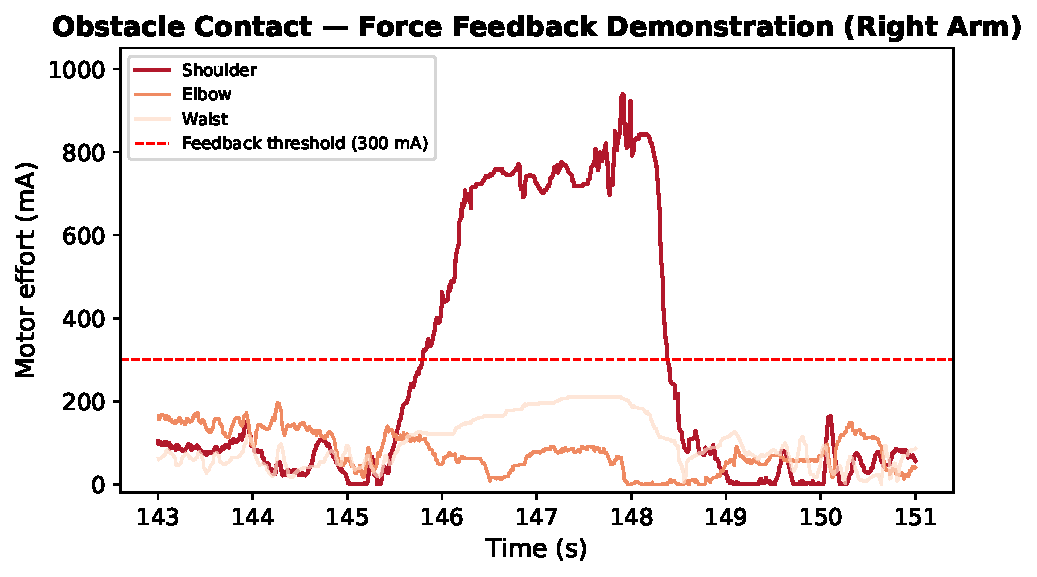
\includegraphics[width=\columnwidth]{figures/effort_contact.pdf}
        \caption{Obstacle contact: shoulder effort exceeds the 300\,mA threshold.}
        \label{fig:effort_contact}
    \end{subfigure}
    \vspace{0.3em}
    \begin{subfigure}[b]{\columnwidth}
        \centering
        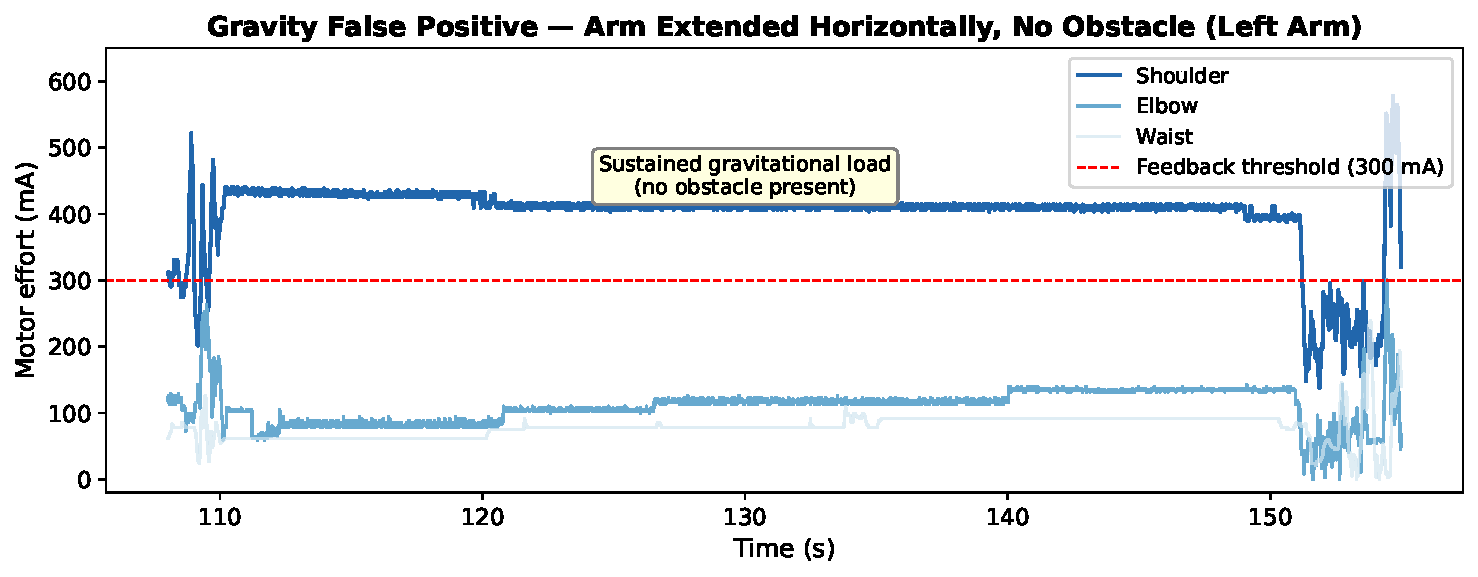
\includegraphics[width=\columnwidth]{figures/effort_gravity.pdf}
        \caption{Gravity false positive: arm extended horizontally with no obstacle, shoulder effort sustained above threshold due to gravitational load alone.}
        \label{fig:effort_gravity}
    \end{subfigure}
    \caption{\textbf{The gravity-contact ambiguity.} Both scenarios produce effort readings above the 300\,mA feedback threshold (dashed line), but only (a) involves actual obstacle contact. Motor current alone cannot distinguish between these cases.}
    \label{fig:effort_comparison}
\end{figure}

We attempted three alternative gating strategies, each addressing a different aspect of the problem.

\textbf{1. Effort derivative gating}: react to the \emph{rate of change} of follower effort rather than its absolute magnitude, hypothesising that contact produces rapid spikes while gravity changes slowly. This filtered some gravity false positives during slow movements but failed on slow or compliant contacts, which produce small derivatives indistinguishable from normal gravity variation. Differentiating the signal also amplifies sensor noise, producing jittery feedback that requires heavy smoothing---reintroducing the latency this approach was meant to avoid.

\textbf{2. Position error detection}: monitor the tracking error between leader and follower joint angles. If the follower falls behind (cannot reach the commanded position), something is blocking it. This partly solves the gravity problem---the follower still tracks under gravitational load, so the error stays small. But feedback is sluggish: error accumulates only \emph{after} the follower physically fails to track, introducing latency that makes the system feel unresponsive.

\textbf{3. Follower velocity detection}: apply resistance only when the follower has near-zero velocity and high effort---the condition indicating a physical obstacle. During motion under gravity, the follower tracks the leader (non-zero velocity), so no false positive occurs. But whenever the operator \emph{pauses} with the arm extended, zero velocity plus high effort from gravity is indistinguishable from zero velocity plus high effort from an obstacle.

The common failure mode is clear: the combined motor current signal $e_j$ includes a gravitational component $g_j(\mathbf{q})$ that depends on joint configuration $\mathbf{q}$. Without computing $g_j(\mathbf{q})$ via inverse dynamics (e.g., Recursive Newton-Euler~\cite{lynch2017modern}), there is no way to isolate the contact force component. This explains why industrial bilateral systems use either dedicated force sensors or accurate dynamics models~\cite{fast_bilateral2025}---and why existing low-cost systems have avoided bilateral feedback entirely.

We consider this characterisation itself a contribution: it establishes a \emph{necessary condition} for robust sensorless bilateral control and explains clearly why commodity servos cannot achieve it without additional computation.

% ===== DISCUSSION =====
\section{Discussion}

\subsection{Comparison with Existing Systems}

Table~\ref{tab:comparison} positions our system against related work. We are, to our knowledge, the only system that combines custom-built scaled followers, bilateral force feedback, and bimanual operation below \$5,000.

\begin{table}[t]
    \centering
    \caption{Comparison with recent low-cost teleoperation systems, with costs normalised to a dual-pair configuration where possible.}
    \label{tab:comparison}
    \small
    \begin{tabular}{@{}lccccc@{}}
        \toprule
        \textbf{System} & \textbf{Cost} & \textbf{Bi.} & \textbf{Bim.} & \textbf{Custom} & \textbf{F/T} \\
        \midrule
        ALOHA~\cite{zhao2023aloha} & \$20k & \ding{55} & \ding{51} & Leaders & \ding{55} \\
        GELLO~\cite{wu_2024_gello} & $<$\$1k\textsuperscript{*} & \ding{55} & \ding{51} & Leaders & \ding{55} \\
        Koch~\cite{koch2024} & \$860\textsuperscript{\dag} & \ding{55} & \ding{55} & Both & \ding{55} \\
        GELLO+Force~\cite{sujit_2025_improving} & \$60k+\textsuperscript{\dag} & \ding{51} & \ding{55} & Leaders & \ding{51} \\
        IGBT~\cite{kanai2025} & N/R & \ding{51} & \ding{55} & \ding{55} & \ding{55} \\
        Bi-ACT~\cite{kobayashi2024} & \$9k & \ding{51} & \ding{51} & \ding{55} & \ding{55} \\
        \textbf{Ours} & \textbf{\$3k} & \ding{51} & \ding{51} & \textbf{Followers} & \ding{55} \\
        \bottomrule
    \end{tabular}
    \vspace{-0.5em}
    \begin{flushleft}
    \footnotesize Bi.~= Bilateral feedback. Bim.~= Bimanual. F/T~= Dedicated force/torque sensor.\\
    \textsuperscript{*}Leader hardware only; requires a separate follower arm (\$10k--\$45k each).\\
    \textsuperscript{\dag}Extrapolated: single-pair cost $\times$\,2.
    \end{flushleft}
\end{table}

\subsection{Lessons for Systems Builders}

Three practical lessons emerged:

\textbf{Integration dominates.} Individual subsystems (teleop, force feedback, collision avoidance) each worked in isolation. Combining four arms into a single ROS~2 graph exposed namespace leaks, udev conflicts, and startup race conditions that took longer to resolve than any individual feature. The gap between ``one pair works'' and ``two pairs work reliably'' was wider than any individual subsystem challenge.

\textbf{Hardware limitations propagate.} The gripper's gearbox friction (the dominant user complaint) is a mechanical property of the XL430 motor, not a software issue. The mixed motor configuration saved 55\% on costs but prevented uniform gravity compensation: XL430 motors lack the current control mode needed for model-based torque estimation. No amount of algorithmic tuning can fix hardware-fundamental constraints. Identifying \emph{which} limitations are hardware-fundamental versus software-addressable saves engineering time.

\textbf{Negative results are load-bearing.} Our three failed force feedback approaches each reveal a different facet of the gravity-contact ambiguity. Documenting \emph{why} they fail provides more actionable guidance than documenting only the approach that worked.

% ===== CONCLUSION =====
\section{Conclusion}

We presented a low-cost bilateral teleoperation system that achieves sensorless force feedback using motor current readings from commodity Dynamixel servos. The system pairs standard PincherX-100 leaders with custom 2$\times$-scaled 3D-printed followers using a torque-tiered motor design, achieving bimanual bilateral teleoperation at $\sim$\$3,000---an order of magnitude cheaper than comparable systems. A user study demonstrated 91.1\% obstacle detection sensitivity and strong perceived learnability (median 7/7). We characterised the fundamental gravity-contact ambiguity that limits sensorless bilateral control and documented three alternative approaches that fail to resolve it, establishing that a dynamics model is a necessary condition for robust force estimation on commodity hardware.

\textbf{Future work.} Gravity compensation via Recursive Newton-Euler inverse dynamics would address the core limitation. Lower gear-ratio motors or series elastic actuators would reduce electromagnetic braking. The system's 1:1 joint-space mapping and ROS~2 architecture make it directly compatible with imitation learning frameworks such as ACT~\cite{zhao2023aloha} and LeRobot~\cite{lerobot2025}, where bilateral demonstrations could improve policy quality~\cite{kobayashi2024}.

\section*{Acknowledgements}
The author thanks Garry Ellard for supervision and guidance throughout this project, and the 22 user study participants. This work was conducted as a final-year undergraduate dissertation at the University of Edinburgh.

\bibliographystyle{IEEEtran}
\bibliography{references}

\end{document}
